\begin{frame}[fragile]{OvertPoly}
    OvertPoly is a \textbf{combinatorial algorithm} for forward reachability analysis of Neural Feedback Systems with \textbf{computational efficiency} comparable to abstraction propagation methods.
\end{frame}

\begin{frame}[fragile]{OvertPoly}
    Our contributions are:
    \begin{itemize}
        \uncover<1->{\item We introduce a \textbf{novel combinatorial abstraction} for nonlinear dynamical systems}
        \uncover<2->{\item Using our abstraction, we define an \textbf{efficient representation} of nonlinear neural feedback systems}
        \uncover<3->{\item We use this representation to define novel algorithms for forward reachability analysis}
        \uncover<4->{\item We demonstrate an \textbf{order of magnitude improvement} in performance compared to the current state-of-the-art}
    \end{itemize}
\end{frame}

\begin{frame}[fragile]{OvertPoly}
    Assumptions:
    \begin{itemize}
        \uncover<1->{\item The nonlinear dynamics are from the class of Extended Algebraic functions}
        \uncover<2->{\item The controller is a ReLU neural network}
    \end{itemize}
\end{frame}

\begin{frame}[fragile]{OvertPoly}
    \begin{figure}
        \begin{center}
            \begin{tikzpicture}
                % Nodes
                \node (plant) [draw, rectangle, minimum width=1.5cm, minimum height=1cm, label=above:{Plant}, fill=green!20] {$f(x)$};
                \node (controller) [draw, below=1.5cm of plant, rectangle, minimum width=1.5cm, minimum height=1cm, label=below:{Controller}] {$\pi(y)$};
                \node (input) [draw, left= 2cm of plant, circle]{$+$};
                \node (noise) [above=0.5cm of input]{$\epsilon$};
                \node (observer) [draw, below right=0.25cm and 1.5cm of plant, rectangle, minimum width=1.5cm, minimum height=1cm, label=right:{Sensor}] {$o(x)$};

                % Edges
                \draw[->] (noise) -- (input);
                \draw[->] (controller) -| (input)node[pos=0.3, yshift=7pt]{$u$};
                \draw[->] (input) -- (plant);
                \draw[->] (plant) -| (observer)node[pos=0.3, yshift=7pt]{$x$};; 
                \draw[->] (observer) |- (controller) node[midway, xshift=7pt, yshift=7pt]{$y$};
            \end{tikzpicture}
        \end{center}
    \end{figure}
\end{frame}

\begin{frame}[fragile]{Polyhedra: Simplices}
    \begin{definition}[$ k $-Simplex]
        A polyhedron $\mathcal{S}$ is a $k$-simplex if it is the convex hull of $k+1$ affinely independent points in $\mathbb{R}^n$.  A polyhedron is a simplex if it is a $k$-simplex for some $k$, and $k$ is called its \emph{dimension}.
    \end{definition}
\end{frame}

\begin{frame}[fragile]{Polyhedra: Simplices}
    \begin{columns}
        \begin{column}{0.3\textwidth}
            \begin{definition}
                A polyhedron $\mathcal{S}$ is a $k$-simplex if it is the convex hull of $k+1$ affinely independent points in $\mathbb{R}^n$.
            \end{definition}
        \end{column}
        \begin{column}{0.7\textwidth}
            \begin{figure}
                \begin{subfigure}{0.3\columnwidth}
                    \begin{tikzpicture}
                        \draw (0,0) -- (3,0);
                    \end{tikzpicture}
                    \caption{$1$-Simplex}
                \end{subfigure}
                \begin{subfigure}{0.3\columnwidth}
                    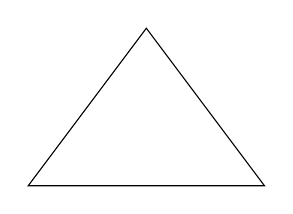
\begin{tikzpicture}
                        \draw (0,0) -- (3,0) -- (1.5,2) -- cycle;
                    \end{tikzpicture}
                    \caption{$2$-Simplex}
                \end{subfigure}
                \begin{subfigure}{0.3\columnwidth}
                    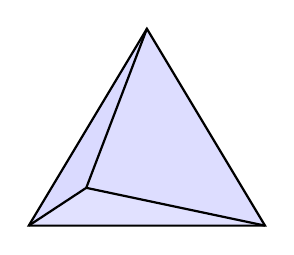
\begin{tikzpicture}
                        % Define vertices in 3D space
                        \coordinate (A) at (0,0,0);
                        \coordinate (B) at (3,0,0);
                        \coordinate (C) at (1.5,2.5,0);
                        \coordinate (D) at (1.5,1.25,2);
                    
                        % Draw filled triangular faces
                        \fill[blue!20,opacity=0.8] (A) -- (B) -- (D) -- cycle;
                        \fill[blue!30,opacity=0.8] (B) -- (C) -- (D) -- cycle;
                        \fill[blue!40,opacity=0.8] (C) -- (A) -- (D) -- cycle;
                        \fill[blue!10,opacity=0.8] (A) -- (B) -- (C) -- cycle;
                    
                        % Draw visible edges
                        \draw[thick] (A) -- (B) -- (C) -- cycle;
                        \draw[thick] (A) -- (D);
                        \draw[thick] (B) -- (D);
                        \draw[thick] (C) -- (D);
                    
                        % Dashed hidden edges
                        \draw[dashed] (A) -- (C);
                    
                    \end{tikzpicture}
                    \caption{$3$-Simplex}
                \end{subfigure}
            \end{figure}
        \end{column}
    \end{columns}
\end{frame}


\begin{frame}[fragile]{Polyhedra: Complexes}
    \begin{definition}[Simplicial $k$-Complex]
        A \emph{simplicial complex} $\mathcal{C}$ is a set of simplices such that:
        \begin{itemize}
        \item Every face of a simplex in $\mathcal{C}$ is also in $\mathcal{C}$
        \item Every non-empty intersection of two simplices $\mathcal{S}_1,\mathcal{S}_2\in\mathcal{C}$ is a face of both $\mathcal{S}_1$ and $\mathcal{S}_2$
        \end{itemize}
        \end{definition}
\end{frame}

\begin{frame}[fragile]{Polyhedra: Complexes}
    \begin{columns}
        \begin{column}{0.3\textwidth}
            \begin{definition}
                \begin{itemize}
                \item Every face of a simplex in $\mathcal{C}$ is also in $\mathcal{C}$
                \item Every non-empty intersection of two simplices $\mathcal{S}_1,\mathcal{S}_2\in\mathcal{C}$ is a face of both $\mathcal{S}_1$ and $\mathcal{S}_2$
                \end{itemize}
            \end{definition}
            
        \end{column}
        \begin{column}{0.7\textwidth}
            \begin{figure}
                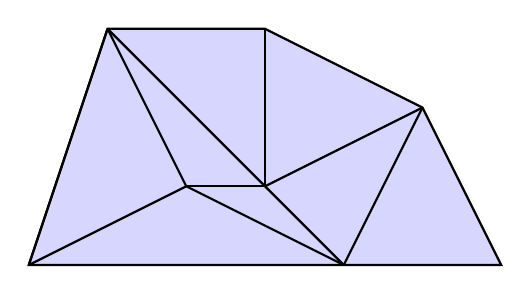
\begin{tikzpicture}
                    % Define points
                    \coordinate (A) at (0,0);
                    \coordinate (B) at (2,1);
                    \coordinate (C) at (4,0);
                    \coordinate (D) at (1,3);
                    \coordinate (E) at (3,3);
                    \coordinate (F) at (5,2);
                    \coordinate (G) at (6,0);
                    \coordinate (H) at (3,1);
                
                    % Fill triangles
                    \fill[blue!20,opacity=0.8] (A) -- (B) -- (D) -- cycle;
                    \fill[blue!20,opacity=0.8] (B) -- (C) -- (H) -- cycle;
                    \fill[blue!20,opacity=0.8] (B) -- (D) -- (H) -- cycle;
                    \fill[blue!20,opacity=0.8] (C) -- (H) -- (F) -- cycle;
                    \fill[blue!20,opacity=0.8] (H) -- (E) -- (F) -- cycle;
                    \fill[blue!20,opacity=0.8] (E) -- (D) -- (H) -- cycle;
                    \fill[blue!20,opacity=0.8] (C) -- (F) -- (G) -- cycle;
                    \fill[blue!20,opacity=0.8] (A) -- (B) -- (C) -- cycle;
                
                    % Draw edges
                    \draw[thick] (A) -- (C) -- (G) -- (F) -- (E) -- (D) -- cycle;
                    \draw[thick] (A) -- (D);
                    \draw[thick] (B) -- (H);
                    \draw[thick] (B) -- (D);
                    \draw[thick] (C) -- (H);
                    \draw[thick] (D) -- (H);
                    \draw[thick] (E) -- (H);
                    \draw[thick] (F) -- (H);
                    \draw[thick] (B) -- (C);
                    \draw[thick] (C) -- (F);
                    \draw[thick] (A) -- (B);
                \end{tikzpicture} 
            \end{figure}
        \end{column}
    \end{columns}
\end{frame}

\begin{frame}[fragile]{Polyhedra: Triangulations}
    \begin{definition}[Point Set Triangulation]
        \uncover<1->{
        If $P$ is a finite set of points in $\mathbb{R}^n$, then a pure simplicial $n$-complex $\mathcal{C}$ is a \emph{point set triangulation of $P$} if $P = \bigcup_{\mathcal{S}\in\mathcal{C}} \mathbf{vert}(\mathcal{S})$ and $\mathbf{conv}(P) = \bigcup_{\mathcal{S}\in\mathcal{S}} \mathcal{S}$.
        \end{definition}}

        \uncover<2->{
        Let $C$ be a closed $n$-ball. We call $C^O$ its open $n$-ball, and $C^S$ the hypersphere forming its surface. We call $V_P(C) = C \cap P$ the vertices of $C$.}

        \uncover<3->{
        If $\mathcal{C}$ is a point set triangulation of $P$, and $\mathcal{S}$ is a $n$-simplex in $\mathcal{C}$, then $C(\mathcal{S})$ is the smallest closed $n$-ball $C$ such that $\mathcal{S} \subseteq C$ and $C^O \cap \mathbf{vert}(\mathcal{S}) = \emptyset$.}

        \uncover<4->{
        $\mathcal{S}$ satisfies the \emph{Delaunay condition} and is called a \emph{Delaunay simplex of $P$} if $V_P(C(\mathcal{S})^O) = \emptyset$.}
        
        \uncover<5->{
        $\mathcal{C}$ is a \emph{Delaunay triangulation} if every $n$-simplex in $\mathcal{C}$ satisfies the Delaunay condition. }
\end{frame}

\begin{frame}[fragile]{Polyhedra: Triangulations}
    \begin{columns}
        \begin{column}{0.3\textwidth}
            \begin{definition}
                If $P$ is a finite set of points in $\mathbb{R}^n$, then a pure simplicial $n$-complex $\mathcal{C}$ is a \emph{point set triangulation of $P$} if $P = \bigcup_{\mathcal{S}\in\mathcal{C}} \mathbf{vert}(\mathcal{S})$ and $\mathbf{conv}(P) = \bigcup_{\mathcal{S}\in\mathcal{S}} \mathcal{S}$.
            \end{definition}
        \end{column}
        \begin{column}{0.7\textwidth}
            \begin{figure}
                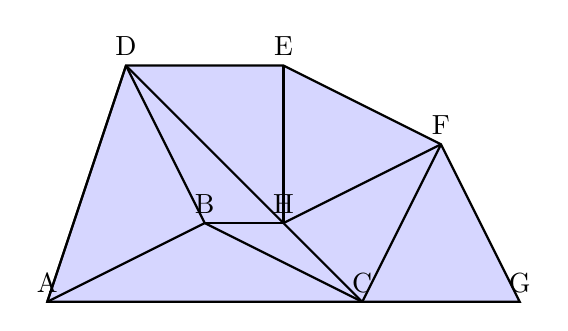
\begin{tikzpicture}
                    % Define points
                    \coordinate (A) at (0,0);
                    \coordinate (B) at (2,1);
                    \coordinate (C) at (4,0);
                    \coordinate (D) at (1,3);
                    \coordinate (E) at (3,3);
                    \coordinate (F) at (5,2);
                    \coordinate (G) at (6,0);
                    \coordinate (H) at (3,1);
                
                    % Fill triangles
                    \fill[blue!20,opacity=0.8] (A) -- (B) -- (D) -- cycle;
                    \fill[blue!20,opacity=0.8] (B) -- (C) -- (H) -- cycle;
                    \fill[blue!20,opacity=0.8] (B) -- (D) -- (H) -- cycle;
                    \fill[blue!20,opacity=0.8] (C) -- (H) -- (F) -- cycle;
                    \fill[blue!20,opacity=0.8] (H) -- (E) -- (F) -- cycle;
                    \fill[blue!20,opacity=0.8] (E) -- (D) -- (H) -- cycle;
                    \fill[blue!20,opacity=0.8] (C) -- (F) -- (G) -- cycle;
                    \fill[blue!20,opacity=0.8] (A) -- (B) -- (C) -- cycle;
                
                    % Draw edges
                    \draw[thick] (A) -- (C) -- (G) -- (F) -- (E) -- (D) -- cycle;
                    \draw[thick] (A) -- (D);
                    \draw[thick] (B) -- (H);
                    \draw[thick] (B) -- (D);
                    \draw[thick] (C) -- (H);
                    \draw[thick] (D) -- (H);
                    \draw[thick] (E) -- (H);
                    \draw[thick] (F) -- (H);
                    \draw[thick] (B) -- (C);
                    \draw[thick] (C) -- (F);
                    \draw[thick] (A) -- (B);
                
                    % Optional: Label vertices
                    \foreach \point/\name in {A/A, B/B, C/C, D/D, E/E, F/F, G/G, H/H}
                        \node[above] at (\point) {\name};
                
                \end{tikzpicture}
            \end{figure}
        \end{column}
    \end{columns}
\end{frame}

\begin{frame}[fragile]{Polyhedra: Bounding Set}
    \begin{definition}[Bounding Set] A \emph{bounding set} is a tuple $\mathcal{B} = \langle n,P, L, U \rangle$, where $n \in \mathbb{N}$, $P$ is finite a set of points in $\mathbb{R}^n$, and $L$ and $U$ are functions from P to $\mathbb{R}$, such that $ L(p) \leq U(p) $ for all $ p \in P. $ The \emph{domain} of $\mathcal{B}$ is defined as $\mathbf{dom}(\mathcal{B})=\mathbf{conv}(P)$.
    \end{definition}
\end{frame}

\begin{frame}[fragile]{Polyhedra: Bounding Set}
    \begin{columns}
        \begin{column}{0.3\textwidth}
            \begin{definition} A \emph{bounding set} is a tuple $\mathcal{B} = \langle n,P, L, U \rangle$. The \emph{domain} of $\mathcal{B}$ is defined as $\mathbf{dom}(\mathcal{B})=\mathbf{conv}(P)$.
            \end{definition}
        \end{column}
        \begin{column}{0.7\textwidth}
            \begin{figure}
                \begin{tikzpicture}
                    \begin{axis}[
                        domain=-1:1, 
                        samples=100, 
                        axis lines=middle, 
                        enlargelimits=true, 
                        xtick=\empty, 
                        ytick=\empty, 
                        xlabel={$x$}, 
                        ylabel={$y$}, 
                        hide axis
                    ]
                    \addplot[blue, thick] {cos(deg(x))};
                    % Rectangle corners
                    \addplot[red, only marks, mark=*] coordinates {(-1,0.5) (1,0.5)};
                    \addplot[blue, only marks, mark=*] coordinates {(-1,1) (1,1)};
                \end{axis}
                \end{tikzpicture}
                                
            \end{figure}
        \end{column}
    \end{columns}
\end{frame}

\begin{frame}[fragile]{Polyhedra}
    \begin{definition}[Polyhedron formed by Bounding Set]
        Let $ \mathcal{B} = \langle n,P,L,U \rangle $ be a bounding set. We define the \emph{vertices} of the bounding set as:
        \[
        V(\mathcal{B}) := \{(p,L(p)) : p \in P\} \cup \{(p,U(p)) : p \in P\}.
        \]
        We define the ($n+1$-dimensional) \emph{polyhedron formed by $ \mathcal{B} $ } as
        \[
        \mathcal{P}(\mathcal{B}) := \mathbf{conv}(V(\mathcal{B})).
        \]
        \end{definition}
\end{frame}

\begin{frame}[fragile]{Polyhedra}
    \begin{columns}
        \begin{column}{0.55\textwidth}
            \begin{definition}
                \[
                V(\mathcal{B}) := \{(p,L(p)) : p \in P\} \cup \{(p,U(p)) : p \in P\}.
                \]
                We define the ($n+1$-dimensional) \emph{polyhedron formed by $ \mathcal{B} $ } as
                \[
                \mathcal{P}(\mathcal{B}) := \mathbf{conv}(V(\mathcal{B})).
                \]
                \end{definition}
        \end{column}
        \begin{column}{0.45\textwidth}
            \centering
            \begin{figure}
                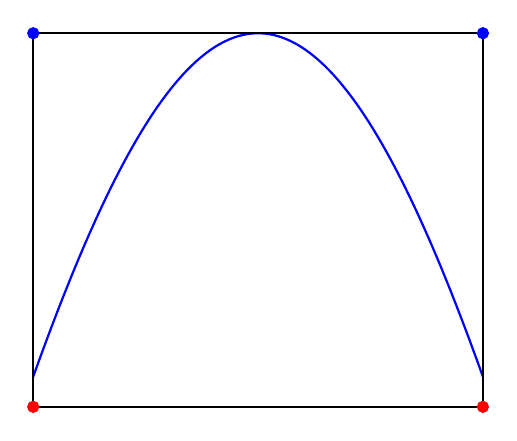
\begin{tikzpicture}
                    \begin{axis}[
                        domain=-1:1, 
                        samples=100, 
                        axis lines=middle, 
                        enlargelimits=true, 
                        xtick=\empty, 
                        ytick=\empty, 
                        xlabel={$x$}, 
                        ylabel={$y$}, 
                        hide axis
                    ]
                    \addplot[blue, thick] {cos(deg(x))};
                    % Rectangle corners
                    \addplot[red, only marks, mark=*] coordinates {(-1,0.5) (1,0.5)};
                    \addplot[blue, only marks, mark=*] coordinates {(-1,1) (1,1)};

                    \draw[thick] (-1,0.5) -- (-1,1) -- (1,1) -- (1,0.5) -- cycle;
                \end{axis}
                \end{tikzpicture}
                                
            \end{figure}
        \end{column}
    \end{columns}
\end{frame}

